%----------------------------------------------------------------------------------------
%	PACKAGES AND OTHER DOCUMENT CONFIGURATIONS
%----------------------------------------------------------------------------------------

\documentclass[a0,portrait]{a0poster}

\usepackage{multicol} % This is so we can have multiple columns of text side-by-side
\columnsep=100pt % This is the amount of white space between the columns in the poster
\columnseprule=3pt % This is the thickness of the black line between the columns in the poster

\usepackage[svgnames]{xcolor} % Specify colors by their 'svgnames', for a full list of all colors available see here: http://www.latextemplates.com/svgnames-colors

\usepackage{times} % Use the times font
%\usepackage{palatino} % Uncomment to use the Palatino font

\usepackage{graphicx} % Required for including images
\graphicspath{{figures/}} % Location of the graphics files
\usepackage{booktabs} % Top and bottom rules for table
\usepackage[font=small,labelfont=bf]{caption} % Required for specifying captions to tables and figures
\usepackage{amsfonts, amsmath, amsthm, amssymb} % For math fonts, symbols and environments
\usepackage{wrapfig} % Allows wrapping text around tables and figures

\begin{document}

%----------------------------------------------------------------------------------------
%   POSTER HEADER 
%----------------------------------------------------------------------------------------

% The header is divided into two boxes:
% The first is 75% wide and houses the title, subtitle, names, university/organization and contact information
% The second is 25% wide and houses a logo for your university/organization or a photo of you
% The widths of these boxes can be easily edited to accommodate your content as you see fit

\begin{minipage}[b]{0.75\linewidth}
\veryHuge \color{NavyBlue} \textbf{Opinion Mining Movie Reviews to Rate Actors} \color{Black}\\ % Title
\Huge\textit{}\\[2cm] % Subtitle
\huge \textbf{David Kale, Scott Shuffler, and Chris Smith}\\[0.5cm] % Author(s)
\huge Appalachian State University Department of Computer Science\\[0.6cm] % University/organization
\Large \texttt{\{kaledj, shuffleres, smithc4\}@email.appstate.edu}\\
\end{minipage}
%
\begin{minipage}[b]{0.25\linewidth}

\includegraphics[width=20cm]{cs6}\\
\end{minipage}

\vspace{1cm} % A bit of extra whitespace between the header and poster content

%----------------------------------------------------------------------------------------

\begin{multicols}{2} % This is how many columns your poster will be broken into, a portrait poster is generally split into 2 columns

\color{DarkSlateGray} % DarkSlateGray color for the rest of the content
%----------------------------------------------------------------------------------------
%   INTRODUCTION
%----------------------------------------------------------------------------------------
\section*{Introduction}

There is vast amounts of unstructured text data on the Internet.  A large chunk of this data exists as user reviews. We use movie review data to try to derive actor ratings from the movies that those actors were a part of.  This project utilizes labeled movie reviews obtained through user input to compute semantic analysis on the words associated with each movie review.  This allows us to use data in order to learn about the movie reviews, and determine how each word used in the review affects the overall review of each movie.  We can use these words, and compute semantic analysis to translate the individual reviews into whether the movie was a good movie, or a bad movie.  This idea can be transformed to work on other datasets of various subjects.  Then, the word analysis and generated movie reviews can be used to construct a model that can be used to rate actors based on the words associated in the actors’ reviews. An overview of our systems architecture is shown in Figure 1. 


%----------------------------------------------------------------------------------------
%   OBJECTIVES
%----------------------------------------------------------------------------------------
\section*{Main Objectives}

\begin{enumerate}
\item We want to use users’ movie reviews in order to analyze them.
\item Using this data, we can learn about movie reviews and how they are structured.
\item By computing semantic analysis on movie reviews, we can determine if a movie was good or bad.
\item We want to generate a model that can be used to rate an actor as good or bad.
\item Rating an actor would be based solely off of reviews of movies that he/she was in.
\end{enumerate}

%----------------------------------------------------------------------------------------
%	DATA AQUISITION
%----------------------------------------------------------------------------------------

\section*{Data Acquisition}

In order to retrieve the data that we need to do this research, we decided to use a premade dataset in order to have ready-to-use data to start with.  We have also implemented a Web scraper in order to retrieve our own data for use at a later date.  This data is stored into a PostgreSQL database, which was created from scratch.  We were able to use the Web scraper to scan a series of Web pages, and then get movie review data.  Afterwards, we were able to merge the concepts of a Web scraper and the concepts of a PostgreSQL database in order to store scraped data into that database.

%------------------------------------------------

\section*{Sentiment Analysis}

The Naive Bayes Classifier is a simple classifier that has used to moderate success in document classification \cite{hand_idiots_2001, mccallum_comparison_1998}. We train our model using Stanfords Large Movie Review Dataset \cite{maas_learning_2011}. An overview of the system is shown in Figure 2.
\newline
\newline
Beginning with a dataset of labeled documents, which in this case are movie reviews labeled as either positive, negative, or neutral, we preprocess each review to make the data more uniform, and to remove useless information \cite{bird_natural_2009}. The preprocessing steps we take are summarized below:
\newline
\begin{itemize}
\item Stop word removal, i.e the removal of words such as “and”,  “the”, and “of”
\item Lemmatization, i.e. combining words that likely have the same meanings into one token, such as combining “includes”, “included”, and, “include” into “include”
\item Removal of non-words, for example newline characters, periods, commas, etc.
\item Finally, we convert all words to lowercase
\end{itemize}
\leavevmode
\newline
After preprocessing, our document is converted into a list of words and with a count of their occurrences. This is commonly referred to as the bag-of-words model. 
\newline
\newline
A Naive Bayes Classifier uses the maximum a posteriori (MAP) decision to rule to assign classes to documents. This rule is given by:
\begin{eqnarray}
C_{map} = argmax_{c\in C} (P(c|d)) = argmax_{c\in C}[P(c)\Pi P(t_k |c)]
\label{eqn:Equation 1}
\end{eqnarray}
where \(t_k\) are the tokens in the document, \(P(c|d)\) is the probability of class given the document, \(P(c)\) is the prior probability of class \(c\), and \(P(t_k|c)\) is the probability of tokens, given class \(c\). We calculate these probabilities using the labeled dataset. 
\leavevmode
\newline

%----------------------------------------------------------------------------------------
%   CONCLUSIONS
%----------------------------------------------------------------------------------------
\section*{Conclusions}

We present an early method for rating actors based on user reviews, which we obtained from the Internet. This idea uses a Web scraper to get movie review data.  Then, the words in these reviews have semantic analysis conducted on them.  This allows us to see whether the word is used in good reviews, bad reviews, or both.  Conducting semantic analysis leads us to using the model generated from the analysis to rate the movies by the words in each review.  Afterwards, we can rate actors after we have a database of generated movie ratings.  This can potentially lead to a system where users review a movie in words, and not numbers.  This would allow for movies, and those who are involved with said movies, to receive number ratings that are solely dictated by the words that people use to describe the movies.  This eliminates the potential skew of number ratings for actors due to partiality or non-movie reasons, such as charity donations.

%----------------------------------------------------------------------------------------
%   END CONCLUSIONS
%----------------------------------------------------------------------------------------

\begin{center}\vspace{1cm}
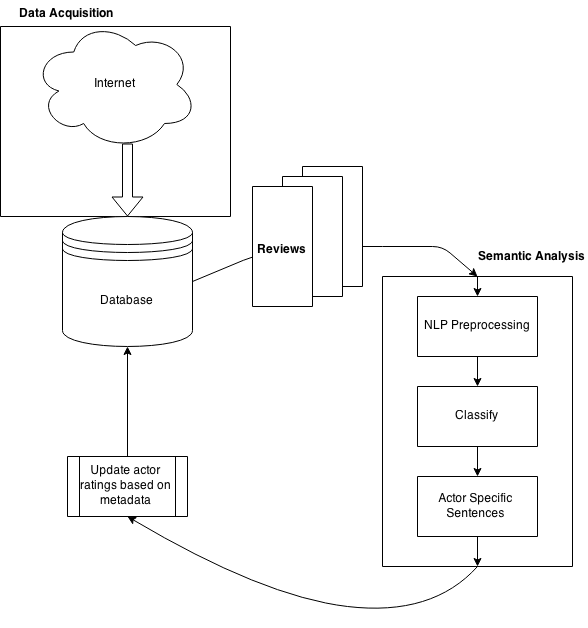
\includegraphics[width=0.8\linewidth]{flow2}
\captionof{figure}{\color{Green} Overall System Flow}
\end{center}\vspace{1cm}


\begin{center}\vspace{1cm}
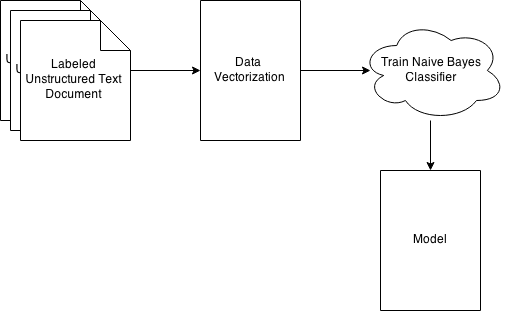
\includegraphics[width=0.8\linewidth]{sentiment}
\captionof{figure}{\color{Green} Sentiment Analysis}
\end{center}\vspace{1cm}


%----------------------------------------------------------------------------------------
%	FORTHCOMING RESEARCH
%----------------------------------------------------------------------------------------

\section*{Future Work}

Ideas for continued research include the following:
\begin{itemize}
\item Figuring out how to utilize occurrences of actors and actresses names in reviews to better rate them.
\begin{itemize}
\item This involves finding a sentence that specifically references the actor/actress and weigh that heavier than the rest of the review.
\end{itemize}
\item Improving the scraper to gather information from various resources, and store the relevant data from those resources.
\item Improving the layout of the PostgreSQL database, as well as the functionality and efficiency of it.
\item Comparing our actor ratings to other reputable sources’ actor ratings.
\end{itemize}

 %----------------------------------------------------------------------------------------
%	REFERENCES
%----------------------------------------------------------------------------------------
\bibliographystyle{ieeetr} % Plain referencing style
\bibliography{chris} % Use the example bibliography file sample.bib

%----------------------------------------------------------------------------------------
%	ACKNOWLEDGEMENTS
%----------------------------------------------------------------------------------------

\section*{Acknowledgements}

Appalachian State S-STEM Program\newline
NSF Supported S-STEM Program\newline
Dr. Rahman Tashakkori

%----------------------------------------------------------------------------------------

\end{multicols}
\end{document}
